\documentclass[aspectratio=169,usenames,dvipsnames]{beamer}
\usepackage{preamble}
\title{Coding for Humanities, week 3}

\begin{document}

\begin{frame}
 \titlepage
\end{frame}

\begin{frame}{Last week}
    \Large
    Sequences

    \vspace{1em}
    Conditions

    \vspace{1em}
    Loops
\end{frame}

\begin{frame}{Plan for today}
 \tableofcontents
\end{frame}

\section{Last week's exercises}
\begin{frame}[fragile]{The Final Quiz}
\dots write code that counts the number of word tokens in
which the letter 'a' is present in a small corpus. You need to do this on the
basis of a frequency distribution of words that is represented by a list of
\texttt{[word, frequency]} pairs.

For example, the word \emph{happening} has an \emph{a} and it occurs
4 times, therefore this word contributes 4 to the total result.
Assign your value to the variable \texttt{number\_of\_words\_with\_a}.

\begin{lstlisting}
frequency_distribution = [['Beg', 1], ["Goddard's", 1], ...]
number_of_words_with_a = 0
# insert your code here
\end{lstlisting}
\end{frame}

\begin{frame}[fragile]{The Final Quiz}
\begin{lstlisting}
frequency_distribution = [['Beg', 1], ["Goddard's", 1], ...]
number_of_words_with_a = 0
for word_and_frequency in frequency_distribution:
    if 'a' in word_and_frequency[0]:
        number_of_words_with_a += word_and_frequency[1]
\end{lstlisting}

\pause
Better:
\begin{lstlisting}
for word, frequency in frequency_distribution:
    if 'a' in word:
        number_of_words_with_a += frequency
\end{lstlisting}
\end{frame}


\subsection{Intermezzo: how to solve problems}
\begin{frame}{How to solve problems}
    \begin{columns}
        \column{0.5\linewidth}
            The Feynman algorithm:
            \begin{enumerate}
                \item Write down the problem.
                \item Think real hard.
                \item Write down the solution.
            \end{enumerate}

            \vspace{1em}
            due to Richard Feynman, \\
            Nobel-prize winning physicist \dots
        \column{0.5\linewidth}\centering
            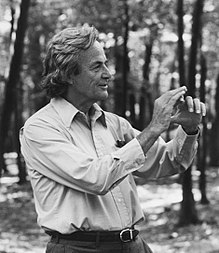
\includegraphics[width=0.6\textwidth]{fig/feynman}

            \vspace{1em} Richard Feynman (1918--1988)
    \end{columns}
\end{frame}

\begin{frame}{How to solve problems}
    \begin{columns}
        \column{0.5\linewidth}
            Pólya (1945), How to solve it:

            \begin{enumerate}
                \item First, you have to \\
                    understand the problem.
                \item After understanding, \\
                    make a plan.
                \item Carry out the plan.
                \item Look back on your work. \\
                    How could it be better?
            \end{enumerate}

            \begin{block}{Stuck?}
            If you can't solve a problem,
            then there is an easier problem you can solve:
            find it.
            \end{block}
        \column{0.5\linewidth}\centering
            
\includegraphics[width=0.6\textwidth]{fig/howtosolveit}

            \vspace{1em} George P\'olya (1887--1985)
    \end{columns}
\end{frame}



\begin{frame}{The 10 exercises}
    \begin{enumerate}
        \item max
        \item max\_of\_three
        \item length
        \item vowel or not?
        \item robber's language \\
            (double every consonant and place an occurrence of ``o'' in between)
        \item sum / multiply
        \item histogram
        \item list of words $\rightarrow$ list of lengths
        \item pangram or not?
        \item 99 bottles of beer
    \end{enumerate}
    \url{https://gist.github.com/andreasvc/60ae38960c1d4c1e1941bf8e96bb2d5f}
\end{frame}

\begin{frame}{How to get better at solving problems?}
    \begin{reference}
        How to become great at just about anything. \url{http://freakonomics.com/podcast/peak/}

        Ericsson, et al 1993. The role of deliberate practice [\dots]. Psych.\ Review
        % Vol. 100. No. 3, 363-406
        (\href{http://graphics8.nytimes.com/images/blogs/freakonomics/pdf/DeliberatePractice(PsychologicalReview).pdf}{link}).
    \end{reference}
    {\centering\Large 
    deliberate practice}

    \vspace{1em}
    Perseverance is more important than talent!
    % Being good at something is NOT about talent

    \begin{enumerate}
        \item \structure{Planning}: Identify your weaknesses
        \item \structure{Dedication}: Practice them
        \item \structure{Repetition}: Practice more \dots
        \item \structure{Reflect} / get feedback
    \end{enumerate}


    %\url{https://en.wikipedia.org/wiki/Practice_(learning_method)#Deliberate_practice}
\end{frame}


\section{Dictionaries}
\frame{\tableofcontents[currentsection]}

\begin{frame}
    \begin{itemize}
        \item Lists are useful when data has a natural order: \\
            get items by their position
        \pause
        \item What if we have lots of data,
            but we need to find it some other way?
    \end{itemize}

    \begin{block}{Example}
    Finding words in a dictionary:

    Too many words to consider one-by-one

    However, due to organization (sorted), can find words quickly
    \end{block}
\end{frame}


\begin{frame}[fragile]{dictionaries}
    \begin{definition}
        A dictionary stores (key, value) pairs, \\
        such that we can quickly find a value given a key.
    \end{definition}
Example, a phone book:
\begin{lstlisting}
>>> coworkers = {'John': 123, 'Mary': 456, 'Alice': 789}
>>> coworkers['Mary']
456
>>> coworkers['Bob'] = 124
\end{lstlisting}

\vspace{1em}
\structure{Aside}: why are dictionaries so fast?\\
Answer: the `magic' of hash tables!
\url{https://dev.to/a_sandrina_p/learning-hash-tables-with-drawings-99o}
\end{frame}

\begin{frame}{Properties of dictionaries}
A dictionary is a mapping of keys to values.

    \begin{itemize}
        \item Looking up a key is fast.
        \item Keys must be immutable (e.g., numbers or strings).
        \item Values can be anything.
        \item Keys are always unique; \\
            re-using a key will overwrite the previous value.
    \end{itemize}
\end{frame}

\begin{frame}[fragile]{Looping over dictionaries}
Looping over a dictionary returns only the keys:
\begin{lstlisting}
data = {'a': 0, 'b': 1}
for key in data:
    print(key)
    print(data[key])
\end{lstlisting}

\pause
Often want both the key and the value:
\begin{lstlisting}
for key, value in data.items():
    print(key)
    print(value)
\end{lstlisting}
\end{frame}

\begin{frame}[fragile]{Tuples}
    \begin{itemize}
        \item Lists are mutable, cannot use as keys in dictionary!
        \item Tuples are similar to lists but are immutable.
    \end{itemize}
Create a tuple with parentheses:

\begin{lstlisting}
couple = ('John', 'Mary')
years_married = {('John', 'Mary'): 3, ('Alice', 'Bob'): 5}
\end{lstlisting}

\pause
Sometimes parentheses can be left out:
\begin{lstlisting}
print(years_married['John', 'Mary'])
for husband, wife in years_married:
    ...
\end{lstlisting}

(technically, the comma creates the tuple \dots)
\end{frame}

\begin{frame}[fragile]{Lists vs dictionaries: practical example}
Two ways of organizing a collection of books:
\begin{lstlisting}
>>> books = ['Tolstoy - War and Peace',
...     'Tolstoy - Anna Karenina',
...     'Dostoevsky - Crime and Punishment',
...     'Dostoevsky - Brothers Karamazov']
\end{lstlisting}

\pause
\begin{lstlisting}
>>> books = {'Tolstoy': ['War and Peace', 'Anna Karenina'],
...     'Dostoevsky': ['Crime and Punishment', 'Brothers Karamazov']}
>>> books['Tolstoy']
...
\end{lstlisting}
Can easily select works by a particular author!
\end{frame}

\begin{frame}{Algorithms + Data structures = Programs}
    \begin{columns}
        \column{0.5\linewidth}
            \begin{itemize}
                \item The way you structure your data is the foundation
                    of your program
                \item The right organization may make the rest of the design
                    obvious
                \item Often a trade-off: particular choices may make one thing
                    easy and another hard
            \end{itemize}
        \column{0.5\linewidth}
            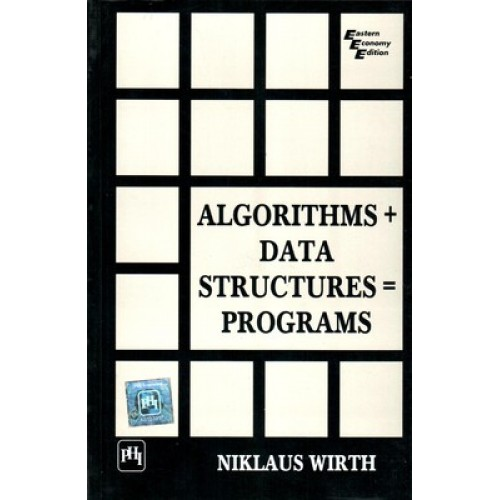
\includegraphics[height=0.6\textheight]{fig/wirth}
    \end{columns}
\end{frame}




\section{Defining functions}
\frame{\tableofcontents[currentsection]}

\begin{frame}{Motivation}
    \begin{itemize}
        \item We've used builtin functions (\texttt{print, len, sorted});\\
            now we'll see how to make our own functions
        \item Why? Modularity; i.e., break down programs into smaller components
            \begin{itemize}
                \item Can create larger, more complex programs
                    from readily understandable building blocks
                \item Functions encapsulate complexity;
                    don't need to understand how a function works to use it
                \item Components are re-usable;
                    write once, use many times
            \end{itemize}
    \end{itemize}
\end{frame}

\begin{frame}[fragile]{Defining functions}
Basic syntax:
\begin{lstlisting}
def function(param1, param2, ...):
    # do something with parameters
\end{lstlisting}

    A function definition has\dots
    \begin{itemize}
        \item A name
        \item Zero or more parameters
        \item An indented block of code
    \end{itemize}
\end{frame}

\begin{frame}[fragile]{Defining a function does not run it}
    \begin{itemize}
        \item Executing a \texttt{def} statement does not run the code!
        \item The function is stored along with its name
        \item Function must be called to run it
    \end{itemize}
    Example:
\begin{lstlisting}
# define function
def greeting():
    print('Hello!')

# call function
greeting()
\end{lstlisting}
\end{frame}

\begin{frame}[fragile]{Function arguments}
    \begin{definition}
        A \structure{parameter} is a value expected by a function

        An \structure{argument} is a particular value for a parameter
            when calling a function
    \end{definition}

    \begin{itemize}
        \item Can pass data to functions using arguments
        \item Below, the argument \texttt{'John'} is assigned \\
            to the parameter \texttt{name} when the function is called
        \item Arguments have a specific order
        \item When calling a function, must use correct number of arguments
    \end{itemize}
Example:
\begin{lstlisting}
def greeting(name):
    print('Hello', name)

greeting('John')
\end{lstlisting}
\end{frame}

\begin{frame}[fragile]{Returning results}
    \begin{itemize}
        \item A function does not need to return a result \\
            In this case,
            \begin{itemize}
                \item the function is used for its \emph{effect};\\
                    it does something (e.g., print text on screen)
                \item The value \texttt{None} is implicitly returned
                        (and usually ignored)
            \end{itemize}
        \item Use \texttt{return ...} to give a result back to the caller
        \item May occur anywhere in the function,\\
                immediately stops execution of the function.
    \end{itemize}

Example:
\begin{lstlisting}
def average(values):
    if not values:
        return None
    return sum(values) / len(values)
\end{lstlisting}
\end{frame}

\begin{frame}{Summary}
    \begin{itemize}
        \item Break programs down into functions \\
            to make them easier to understand.
        \item Define a function using \texttt{def} with a name, parameters,\\
            and a block of code.
        \item Defining a function does not run it.
        \item Arguments in a call are matched to parameters in definition.
        \item Functions may return a result to their caller using \texttt{return}.
    \end{itemize}
\end{frame}




% Talk about reading files?

\section{Text processing}
\subsection{Motivation}
\frame{\tableofcontents[currentsection]}

% \begin{frame}{Why count words?}
%     Linguistic Inquiry and Word Count (LIWC, Pennebaker)
%     \begin{itemize}
%         \item Counts words in 80 categories:
%             \begin{itemize}
%             \item linguistic (e.g., first-person singular pronouns, conjunctions),
%             \item psychological (e.g., anger, achievement),
%             \item topical (e.g., leisure, money)
%             \end{itemize}
%         \item Uses word counts to analyze personality or psychological state
%         \item \url{http://secretlifeofpronouns.com/}
%         \item \url{https://www.scientificamerican.com/article/you-are-what-you-say/}
%     \end{itemize}
% \end{frame}

\begin{frame}{Distant Reading}
\begin{reference}
\href{https://www.versobooks.com/books/261-graphs-maps-trees}{
Moretti (2005) Graphs, maps, and trees}

\end{reference}
\begin{columns}
\column{0.5\linewidth}
        \begin{definition}
        \structure{Distant reading}:
        taking a bird's eye view of a corpus using computational tools
        \end{definition}
    \begin{itemize}
        \item goal: find patterns, trends
        \pause
        \item example: Rybicki et al (2016): computational stylistics and text analysis
    \end{itemize}
\column{0.5\linewidth}
    \onslide
    
\includegraphics[width=\linewidth]{fig/catbooks.jpg}
\end{columns}
\end{frame}


\begin{frame}{What kind of patterns and trends?}

	\pause
	\emph{try the simplest thing that could possibly work}\texttrademark

	\pause
	\vspace{2em}
	\centering
	text $\rightarrow$ word counts

    \pause
    \vspace{2em}
    ``All models are wrong, but some are useful'' --- George Box
\end{frame}


\begin{frame}
\frametitle{Bag-of-Words model}
	\begin{definition}
		\structure{Bag-of-Words (BOW)} model:
		    summarize a collection of texts by their word counts
	\end{definition}
    \vspace{1em}
    
    \begin{columns}
    \column{0.6\textwidth}
	Example:
	
	\begin{tabular}{lrrrrr}
	Author      & \em Shall & \em~I & \em compare & \em thee & \dots \\ \midrule
	Shakespeare &     1 & 1 &       1 &    1 & \dots \\
	Me          &     0 & 9 &       0 &    0 & \dots \\
	\pause
	??          &     0 & 7 &       0 &    0 & \dots \\
	\end{tabular}
	
	\vspace{1em}
    (usually, relative frequency is used)
    \column{0.4\textwidth}\pause
        \hspace{1em}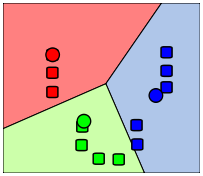
\includegraphics[width=0.7\textwidth]{fig/vsm.png}
    \end{columns}
\end{frame}

\begin{frame}{Why count words?}
    Authorship attribution
    \begin{itemize}
        \item Given a work with unknown/disputed authorship,
        \item Compare its word frequencies with works of possible authors
        \item Function words leave a remarkably strong stylistic `fingerprint'
    \end{itemize}

    \pause
    Examples:
    \begin{itemize}
        \item In 2015 the play Double Falsehood was attributed to Shakespeare
                (instead of John Fletcher)
            \url{http://www.latimes.com/science/sciencenow/la-sci-sn-shakespeare-play-linguistic-analysis-20150410-story.html}

        \item Patrick Juola. 2015. The Rowling Case: A Proposed Standard Analytic Protocol for Authorship Questions. %Digital Scholarship in the Humanities, vol. 30, supp. 1.
            \url{https://doi.org/10.1093/llc/fqv040}
        \item The unmasking of Elena Ferante
            \url{https://www.newyorker.com/culture/cultural-comment/the-unmasking-of-elena-ferrante}
            \\
            {\small\url{https://www.researchgate.net/publication/320131096_Elena_Ferrante_Unmasked}}
        % \item \url{https://www.publicbooks.org/authorship-after-ai/}
    \end{itemize}
\end{frame}

\begin{frame}{Why count words?}
    \begin{reference}
        \href{http://www.infotext.unisi.it/upload/rybickihoovereder_with_figures.pdf}{Rybicki, J., Eder, M., \& Hoover, D. (2016). Computational stylistics and text analysis (link)}
    \end{reference}
    Stylistic analysis
    \begin{itemize}
    \item Collaborative authorship of a novel:\\
        who wrote what?
            % Classification
    \item Six narrators in Woolf's \emph{The Waves}:\\
        differentiation of characters by gender and age
            % Clustering
    \item Vocabulary of 366 student essays wrt.\ grades:
        which words are characteristic of good and bad essays?
            % Keywords
    \item Diachronic analysis of 1000 novels \\
        (diachronic: change over time)
            % Network analysis
    \end{itemize}
\end{frame}


\subsection{Cleaning and preprocessing text}
\begin{frame}{Goal: text $\rightarrow$ words}
    For basic text analysis,

    Want to consider only word frequencies of a text

    \vspace{1em}
    Basic approach:
    \begin{enumerate}
        \item Simplify text: lower case, remove punctuation
        \item Identify words / word boundaries
        \item Count words to get frequencies
    \end{enumerate}
\end{frame}


\begin{frame}[fragile]{Upper and lower case}
    \begin{itemize}
        \item To the computer, these
            are three completely different words!

            \texttt{'The', 'the', 'THE'}
        \item Often, we don't want to make this distinction when counting
        \item Solution: case folding
    \end{itemize}
    \pause
\begin{lstlisting}
In: text = 'HeLlO WoRlD'
In: cleaned = text.lower()
In: cleaned
Out: 'hello world'
\end{lstlisting}
\end{frame}

\begin{frame}[fragile]{Punctuation}
    \begin{itemize}
        \item Similarly, punctuation should be separated from words
        \item \dots or eliminated completely
        \item Can use functionality similar to "find \& replace" for this
    \end{itemize}
    \pause
\begin{lstlisting}
In: text = "Forsooth, 'tis true!"
In: cleaned = text.lower()
In: cleaned = cleaned.replace('!', '')
In: cleaned = cleaned.replace(',', '')
In: cleaned
Out: 'forsooth tis true''
\end{lstlisting}
\end{frame}


\begin{frame}[fragile]{Tokenization}
 \begin{itemize}
  \item task: splitting a string up into tokens
  \item \structure{tokens} are (1) words, (2) punctuation marks, (3) various other things
  \item first and most basic step in text analysis,
        should be done automatically
  \item various algorithms and tools exist, none is perfect
  \item Where to split text? Most important cues: whitespace, punctuation
 \end{itemize}
 \begin{lstlisting}
>>> tokenize('"Hark! A vagrant," he said.')
['"', 'Hark', '!', 'A', 'vagrant', ',', '"', 'he', 'said', '.']
 \end{lstlisting}
\end{frame}

\begin{frame}[fragile]{Tricky tokenization cases}
One or two tokens?
 \begin{itemize}
  \item \structure{prime minister}
  \item \structure{New York}
  \item \structure{I'm}
 \end{itemize}

\pause
\vspace{1em}
More tricky cases:
\begin{verbatim}
John's bike
New York-based
nineteenth- and twentieth-century writers
(SAM)-missile launchers
i.e.  Ph.D. &c.
;-) :))) #yolo#lit#hashtag
https://en.wikipedia.org/wiki/Bicycle
8-Cyclopentyl-1,3-dimethylxanthine
\end{verbatim}
\end{frame}




% \begin{frame}[fragile]{The split method}
% We can turn a string into a list of strings
% by splitting on a `separator':
% \begin{lstlisting}
% In: quote = "Frankly, my dear, I don't give a damn."
% In: quote.split(",")
% Out: ['Frankly', ' my dear', " I don't give a damn."]
% \end{lstlisting}
% 
% \pause
% If we don't give a character, splits on whitespace:
% \begin{lstlisting}
% In: quote.split()
% Out: ['Frankly,', 'my', 'dear,', 'I', "don't", 'give', 'a', 'damn.']
% \end{lstlisting}
% \end{frame}
% 
% 
% \begin{frame}[fragile]{Putting a list of strings back together as one string}
% \begin{lstlisting}
% In: ''.join(sorted(letters))
% 'cdo'
% \end{lstlisting}
% Equivalent of:
% \begin{lstlisting}
% In: 'c' + '' + 'd' + '' + 'o'
% \end{lstlisting}
% 
% \texttt{sep.join(seq)} is the opposite of \texttt{str.split(sep)}
% \end{frame}


\begin{frame}{Word forms}
    Should we count these separately:

    \vspace{1em}
    \texttt{walk, walks, walked, walking, \dots}

    \vspace{1em}
    \begin{itemize}
    \item Recognizing that these are forms of the same word
    is called \structure{lemmatization}.

    \item Requires language-specific tools.

    \item Most work does not apply this step for simplicity,\\
        and forms may contain useful distinctions.
    \end{itemize}
\end{frame}

\begin{frame}{Eliminating classes of words}
    For some applications, want to ignore certain words:
    \begin{itemize}
        \item Function words / stop words (highly frequent words that do not carry meaning)
        \item Names
    \end{itemize}

    But in other applications, these are the most interesting words!
\end{frame}

% \begin{frame}[fragile]{Counting}
% How to count the number of 'a's in a string?
% \begin{lstlisting}
% word = 'banana'
% count = 0
% \end{lstlisting}
% \pause
% \begin{lstlisting}
% for letter in word:
%     if letter == 'a':
%         count += 1
% print(count)
% \end{lstlisting}
% \end{frame}
% \begin{frame}[fragile]{Is there a better way?}
% Yes! Look at documentation on strings:
%
% \begin{block}{\texttt{str.count(sub[, start[, end]])}}
%     Return the number of non-overlapping occurrences of substring \emph{sub}
%     in the range \emph{[start, end]}.
%     Optional arguments start and end are interpreted as in slice notation.
% \end{block}
%
% See \url{http://docs.python.org/3/library/stdtypes.html#string-methods}
%
% \pause
% \begin{lstlisting}
% word = 'banana'
% print(word.count('a'))
% \end{lstlisting}
% \end{frame}

\begin{frame}{More complicated searches and substitutions}
What if we want to find or replace \dots
\begin{itemize}
    \item Words that start or end with certain letters
    \item Words that (do not) contain certain letters
    \item Words with a certain number of letters or substrings
    \item Words that follow a certain structure
\end{itemize}

Learn \structure{regular expressions}:\\
%\url{https://docs.python.org/3/howto/regex.html}
\url{https://www.programiz.com/python-programming/regex} \\
% \url{https://www.datacamp.com/community/tutorials/python-regular-expression-tutorial}

\vspace{1em}
Takes time to learn, but extremely powerful!
\end{frame}

\begin{frame}[fragile]{Regular expression example}
\begin{lstlisting}
def pagenumbers(text, threshold=50):
    """Strip lines that contain only a number.

    Only applied when a threshold is reached,
    to avoid removing chapter numbers."""
    # remove page numbers of the form <23> or |23| in running text;
    text = re.sub(r'<[0-9]+>|\|[0-9]+\|', '', text)
    # Remove other page numbers only when on their own line.
    pagenumber = re.compile(r'\n+[\t ]*-*[\t ]*[0-9]+[\t ]*-*[\t ]*\n+[\f\v]*')
    if len(pagenumber.findall(text)) >= threshold:
        return pagenumber.sub('\n', text)
    return text
\end{lstlisting}
\end{frame}

\begin{frame}{Text encoding}
    \begin{itemize}
        \item Text with accented or non-Western characters or emojis \\
            has an \structure{encoding}
        \item Encoding must be specified correctly when reading and saving!
        \item Always use the Unicode character set with UTF-8 encoding! \\
            (Default for Python and many programs)
        \item Might be a problem with older datasets or Windows programs.
    \end{itemize}
  
    Example encoding problem:

    \begin{columns}
    \column{0.5\linewidth}\centering
         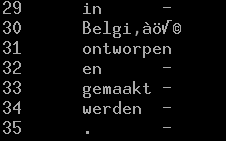
\includegraphics[width=0.5\textwidth]{fig/encodingissue}
    \column{0.5\linewidth}
        Should read:\\
        \texttt{30   Belgi\"e}
        \vspace{3em}
    \end{columns}

    \vspace{1em}
    For more information: \url{https://docs.python.org/3/howto/unicode.html}
\end{frame}

\begin{frame}{Summary}
    \begin{itemize}
        \item Text is often messy
        \item Cleaning: handle punctuation, case, removing words
        \item Tokenization: split text in list of tokens
        \item Count words, analyze
    \end{itemize}
\end{frame}

\begin{frame}{Background reading}
    \begin{itemize}
        \item Downey ch.\ 3, 6, 11, 14
        \item and/or Zelle sec.\ 5.9, ch.\ 6
        \item Watch youtube tutorials of "Hacking the Humanities" episode 10--12:
            {\small \url{https://www.youtube.com/playlist?list=PL6kqrM2i6BPIpEF5yHPNkYhjHm-FYWh17}}
    \end{itemize}
\end{frame}
\end{document}
